% Budget/contract: 1.1 pages. Main contribution section. Define task, label
% construction with no-trade band, chronological day-block splits with zero
% train/eval target-window overlap (no purge/embargo gap),
% dummy floors, readout metrics, predeclared criteria, validation-budget ledger,
% and Fig 1. Values from claims ledger v1.13: horizon_k=9 bars, band=3.0 bps;
% train 1998-01-02 -> 2013-09-16, validation -> 2017-01-25 (end exclusive).
\section{Task and Evaluation Protocol}\label{sec:protocol}

The protocol freezes the label, splits, baselines, readout metric, and decision
criteria before the first model score. Any reported margin is therefore prespecified, not
a post hoc choice. Split-boundary controls fix which rows can be scored, and a
validation-budget ledger records the logged route-scoring contact behind the
margin
\cite{kapoor2023leakage,lopezdeprado2018advances}. We demonstrate it on a single
near-null case with no known-signal positive control, so its power to separate
signal from noise is asserted by construction, not shown here.

\subsection{Task}

We frame this as drop-neutral binary intraday direction classification on
5-minute bars, resampled from 1-minute data for five US large-cap equities
(CSCO, JPM, KO, MSFT, WMT). Each prediction unit is one ticker and one completed
5-minute target bar, scored up or down over a fixed forward horizon. Any edge this
procedure retains is classification evidence, not economic value.

\subsection{Label}

Each row's target is the sign of the 9-bar-ahead forward return. With \(\theta\)
the no-trade band in return units, a target row is
labeled up when the forward return exceeds \(+\theta\) and down when it falls
below \(-\theta\); a row inside the band is flagged invalid and dropped. We fix
the band at \(3.0\) bps, which removes
near-flat moves whose direction is dominated by noise
\cite{xu2018stock,sun2017predicting} and changes the label distribution relative
to all bars \cite{zadrozny2004learning}. It also defines the per-day activity
proxy used in a later conditional diagnostic, a limitation rather than a result.
Labels and windows are day-local and per-ticker: neither the horizon window nor a
label crosses a trading-day boundary or a ticker. The remaining up/down rows are
the only supervised rows; no-trade rows are not a third class and are not imputed.

\subsection{Chronological splits}

Chronological day blocks define the partitions, fixed by the Stage~00 freeze
\cite{hyndman2021forecasting}. Train runs from 1998-01-02 to 2013-09-16
(end exclusive); official validation runs from 2013-09-16 to 2017-01-25
(end exclusive); the holdout is closed from 2017-01-25. No stage in the
validation pipeline reads or scores a post-2017 bar; the run manifest records
holdout contact as false. The guarded walk-forward readout there
(Section~\ref{sec:guarded}) opens this segment only after the model is frozen, so
it is a non-independent confirmation of the frozen primary, not a clean test. Because
every window and horizon stays inside one trading day, the last train and first
evaluation target windows cannot straddle the cut or share rows. The template
deliberately substitutes this within-day locality for purge and embargo, and we
apply neither. Cross-day serial dependence therefore stays intact, a limitation
rather than a solved problem. Preprocessing that learns statistics is fit on train
rows only and applied unchanged to validation. The feature window \(w = 20\) is likewise fixed by a
train-inner feature and window search (Section~\ref{sec:setup}), not as a
validation-tuned readout parameter.

\subsection{Baselines}

Every model score is reported against same-row trivial baselines on the identical
target rows within each readout domain. The validation criteria use a stratified
dummy, which samples from the empirical train label prior, and a majority
baseline, which always predicts the most frequent train label. The stratified
dummy fixes a same-row label-prior \macrofone{} floor for the drop-neutral
target. A margin over it means ``above train-prior guessing'' on the same rows;
it does not by itself rule out serial structure or microstructure effects.

\subsection{Readout metric and predeclared criteria}

The model-versus-dummy margin is measured in \macrofone{} on the drop-neutral
up/down target. The decision criteria were predeclared in the dated protocol
before any readout~\cite{hofman2023preregistration} and are evaluated on the predeclared TCN
primary. On the validation split it passes
when its \macrofone{} delta is positive over both the stratified dummy and the
majority baseline, and at least three of the five tickers are positive (a floor,
not the achieved count). These are deliberately weak floors: predeclaration only
prevents moving the bar after the fact; it does not make the bar discriminating.
The guarded walk-forward readout carries its own separate, also weak, predeclared
stability bar. Neither readout is a model-selection event, and no final model is
selected.

\subsection{Validation-budget ledger}

Each readout contact with the official validation split is counted and tier-tagged
in a validation-budget ledger, and every such contact carries
\texttt{for\_selection} set to false. This makes logged route contacts traceable
within the route and bounds disclosed reuse of the official validation split; it
is not an external timestamp.
The ledger later reports \numseeds{} official-validation seed-candidate scoring
events and 56 guarded scoring events. The paper also keeps three evidence domains separate, each
reported only within its own domain. These are the official validation readout over \numseeds{} seeds, the
train-inner control comparisons, and the guarded non-independent
walk-forward readout, also scored under the two prespecified seeds. Every reported
number names its domain, and no sentence mixes them.

Figure~\ref{fig:protocol-timeline} summarizes the timeline and the freeze ordering.

\begin{figure}[t]
  \centering
  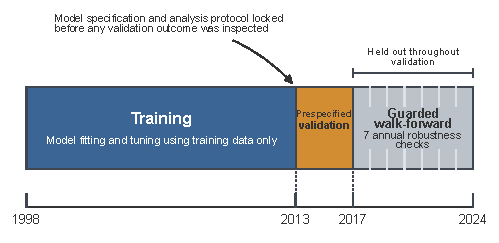
\includegraphics[width=\linewidth]{figures/fig_protocol_timeline}
  \Description{A single-row, to-scale timeline from 1998 to 2024 with three
    contiguous eras: a wide blue Training band labelled model fitting and
    tuning using training data only, a narrow amber Prespecified validation
    band, and a neutral-grey Guarded walk-forward era holding seven robustness
    checks, the final block longer than the 12-month width of the others. The
    phase and action labels are written inside the
    colored bands, while the lower axis carries only the boundary years 1998,
    2013, 2017, and 2024, with guide lines linking the 2013 and 2017 split
    boundaries to the colored bands. An arrow states that the model
    specification and analysis protocol were locked before any validation
    outcome was inspected. A bracket over the post-2017 era states that it was
    held out throughout validation. The caption states the freeze ordering,
    validation use, and non-independence limitation; split sizes and
    frozen-decision details are reported in the surrounding protocol and dataset
    table.}
  \caption{Protocol timeline and freeze ordering for the drop-neutral up/down
    direction task. Chronological day-blocks define training
    (1998-01-02--2013-09-16), one official validation readout
    (2013-09-16--2017-01-25), and a guarded post-2017 era. Model specification
    and analysis protocol are locked before validation; validation is
    prespecified, not tuning or model selection, and no final model is chosen.
    The post-2017 region was untouched during validation; the guarded
    walk-forward checks confirm a frozen model over non-independent periods, so
    they are not future-blind or independent holdout tests.}
  \label{fig:protocol-timeline}
\end{figure}
